\documentclass[a4paper]{article}

\usepackage[english]{babel}
\usepackage[utf8]{inputenc}
\usepackage{float}
\usepackage{amsmath}
\DeclareMathOperator*{\Max}{Max}
\usepackage{amssymb}
\usepackage{pdfpages}
\usepackage{varwidth}
\usepackage{graphicx}
\usepackage{csquotes}
\usepackage{dirtytalk}
\usepackage{hyperref}
\usepackage{xcolor}
\usepackage{listings}
\lstset{
  basicstyle=\ttfamily,
  columns=fullflexible,
  frame=single,
  breaklines=true,
  postbreak=\mbox{\textcolor{red}{$\hookrightarrow$}\space},
}
\newcommand\todo[1]{\textcolor{red}{TODO: #1}}

\title{REI602M Machine Learning: Allstate Claims Severity}

\author{Eggert Jon Magnusson and Thor Tomasarson}

\date{\today}

\begin{document}
\maketitle

\begin{abstract}
The goal of this assignment is to find a good regression model that predicts the severity or loss for each insurance claim made by customers of the Allstate insurance. The dataset used in this report can be found at \url{https://www.kaggle.com/c/allstate-claims-severity}.

\begin{displayquote}
Dataset Information: \\\\
\say{Allstate is currently developing automated methods of predicting the cost, and hence severity, of claims. In this recruitment challenge, Kagglers are invited to show off their creativity and flex their technical chops by creating an algorithm which accurately predicts claims severity. Aspiring competitors will demonstrate insight into better ways to predict claims severity for the chance to be part of Allstate‘s efforts to ensure a worry-free customer experience.}
\end{displayquote}

\end{abstract}

\section{Introduction}

There are quite many methods available that serve as regression models. The methods tested out in this report are: \\

\begin{varwidth}[t]{.5\textwidth}
    Linear:
    \begin{itemize}
        \item Linear Regression
        \item Ridge
        \item Lasso
        \item Elastic-Net
    \end{itemize}
\end{varwidth}
\hspace{4em}
\begin{varwidth}[t]{.5\textwidth}
    Non-linear:
    \begin{itemize}
        \item K-Neighbors Regression
        \item Support Vector Regression
        \item Bagging Regression
        \item Random Forest Regression
        \item Extra Trees Regression
        \item Gradient Boosting Regression
        \item MLP (Neural Network)
    \end{itemize}
\end{varwidth} \\\\
These models require different kind of preprocessing of the data in order to be efficient. The need for preprocessing ranges from next to no preprocessing up to extensive investigation of each attributes contribution to the output. The dataset it self is well structured CSV files with more than 188’000 “labeled” data sets and consists of 130 attributes of which 14 are continuous and 116 are categorical.

To start with each of these models were tested out with default parameters to get a feel of there potential. Then a extensive evaluation of different hyper-parameters where tested out for the more promising methods with various degree of preprocessing.

All experiments where done with Python in JuPyter, the methods tested where gotten from the Scikit-Learn library except for the neural network that was implemented with TensorFlow.

% 0.5 til 1 bls.
% * Hvað var gert?
% * Hvers vegna?
% * Hvernig?

\section{Implementation}

The work methodology for each regression model was as follows:
\begin{enumerate}
  \item Read the data in to memory and split it to training and test datasets
  \item Preprocess the data
  \item Test out various hyper-parameters
  \item Evaluate the results with test data
  \item Go back to step 2 or 3, until decent results were obtained
\end{enumerate}
For all of these models the test error was evaluated with mean absolute error (MAE) \ref{eq:0} on separate test data.
\begin{equation} \label{eq:0}
|y - \hat{y}|
\end{equation}
Where $y$ is the actual output and $\hat{y}$ is the predicted output.

\subsection{Linear models}
The linear models are sensitive to the input data. They can perform badly if the input data contains correlated attributes as they expect a normally distributed output.

The basic ideal behind the linear models are that they are solving equation~\ref{eq:1}, which is minimizing $L^2$-norm error of a hyperplane.  
\begin{equation} \label{eq:1}
\min_{\omega\in\mathbb{R}^p}||X\omega - y||_2^2
\end{equation}
Where $X$ is the input data, $p$ is the input dimension, $\omega$ are the model parameters and $y$ is the output data, in our case it is ‘loss’. \\\\
\textbf{Linear regression} simply solves for equation \ref{eq:1} with no regularization of the model parameters. This can lead to severe overfitting of the training data and is sensitive the input data used. \\\\
\textbf{Ridge regression} adds in the $L^2$-norm penalty, which changes the problem to minimizing the error with equation~\ref{eq:2}.
\begin{equation} \label{eq:2}
\min_{\omega\in\mathbb{R}^p} \{||X\omega - y||_2^2 + \lambda_2*||\omega||_2^2 \}
\end{equation}
This forces the model parameters to be as small as possible.\\\\
\textbf{Lasso regression} adds in the $L^1$-norm penalty, and is thus solving for minimum of equation~\ref{eq:3}
\begin{equation} \label{eq:3}
\min_{\omega\in\mathbb{R}^p}  \{||X\omega - y||_2^2 + \lambda_1*||\omega||_1\}
\end{equation}
This forces some of the model parameters to be zero, thus removing unneeded or correlated attributes. \\\\
\textbf{Elastic-Net} combines the regularization of both Ridge and Lasso, see equation~\ref{eq:4}. By that it combines the effect of $L^1$-norm to force unneeded parameters to zero and the $L^2$-norm to hold of a little information from that parameter (not setting to complete zero).
\begin{equation} \label{eq:4}
\min_{\omega\in\mathbb{R}^p}  \{||X\omega - y||_2^2 + \lambda_1*||\omega||_1 + \lambda_2*||\omega||_2^2\}
\end{equation}

All these models are solving for minimum of error with $L^2$-norm, this counters the objective which is to find model which minimizes the absolute mean error ($L^1$-norm).

\subsection{Non-linear models}
The non-linear models differ quite a lot on what there objective is and how they achieve it. \\\\
\textbf{k-nearest neighbors} learns the dataset and estimates value predictions based on averaging the k nearest neighbors output values. \\\\
\textbf{Support vector regression} solves for the “soft margin” with slack variables $\xi_n$ and $\xi_n^*$ that allow for violation on both sides. The problem can be formulated as:
\begin{align} \label{eq:5}
    &\min_{\omega} \{\frac{1}{2}\omega^T\omega + C\sum_i(\xi_n + \xi_n^*)\} \notag \\
&\text{subject to} \notag \\
    & \forall n : y_n - (x_n^T\omega + b) \leq \epsilon + \xi_n \notag \\
    & \forall n : (x_n^T\omega + b) - y_n\leq \epsilon + \xi_n^* \notag \\
    & \forall n : \xi_n^* \geq 0, \forall n : \xi_n \geq 0 \notag \\ \notag
\end{align} % https://se.mathworks.com/help/stats/understanding-support-vector-machine-regression.html
where the subscript $n$ denotes the $n$-th item in the dataset.
\subsubsection{Decision Trees}
The decision trees (DT) models considered here improve upon the classical week learner DT with a voting scheme. The voting scheme fits multiple regression DT and then aggregate there results to achieve higher precision. \\\\
\textbf{Bagging Regression} models each decision tree with a random subset of the original data. \\\\
\textbf{Extra Trees Regression} models multiple stochastic decision trees where each DT only models for random $D$ variables and a random value is selected for each split. \\\\
\textbf{Random Forest Regression} combines the effects of both bagging and extra trees, by modeling decision trees on random subset of the data and with random $D$ variables. \\\\
\textbf{Gradient Boosting Regression} starts with a single small decision tree and subsequent DT predict the error residual of the previous predictions.
\subsubsection{Neural Network}
\textbf{Multilayer perceptron (MLP)} a feedforward artificial neural network with ReLu activation function \ref{eq:7} and an MAE objective function.
\begin{equation} \label{eq:7}
ReLu(x) = x^+ = max(0, x)
\end{equation}

\subsection{Preprocessing}
The preprocessing methods used for our results were for example:
\begin{itemize}
    \item Visual inspection of attribute (frequency, mean, std, distribution)
    \item Correlation checks
    \item Dimension reduction methods (PCA and NMF)
\end{itemize}
Dimension reduction with \textbf{Principal component analysis} (PCA) is a way of extracting the top $n$ most variance explaining components in the dataset.

While dimension reduction with \textbf{Non-Negative Matrix Factorization} (NMF) “compresses” the dataset $X$ in to two smaller matrices $X=WH$, where W forms the vector basis of $X$. Care must be taken when using NMF since it is only applicable to non-negative dataset, which fortunately is the case for this dataset.


% * Lýsing á aðferðafræði.
% * Stutt lýsing á þeim reikniritum sem eru notuð: flokkarar, aðhvarfsgreiningarlíkön, t-SNE, þyrpingagreining, …
% * Stutt lýsing á gagnasafni/söfnum.
% * Hvernig nákvæmni spálíkana er metin.
% * Hvernig gildi á “hyperparametrum” eru valin
%
% Nákvæmni í lýsingu á að miðast við að samnemendur ykkar í REI602M geti endurtekið tilraunirnar án teljandi vandræða

\section{Results}
Investigation on the dataset lead to few interesting facts, which are listed here:
\begin{itemize}
    \item The output data (‘loss‘) is highly skewed to the left, see figure~\ref{fig:loss}
    \item No value is missing
    \item All continuous attributes are on the [0, 1] interval
    \item None of the continuous attributes correlate with the output (all with $|\rho| < 0.1$)
    \item High correlation among some of the continuous attributes, see figure~\ref{fig:con-corr}
    \item High correlation among some of the categorical attributes, eight pairs have $r_s > \tau > 0.90$
    \item The highest correlated categorical attribute with the output is ‘cat80’ with $\tau=-0.38$, nine others with $|\tau| \geq 0.2$
\end{itemize}
Here above the symbols $\rho$, $\tau$ and $r_s$ denote Pearson, Kendall's tau and Spearman’s rank correlation coefficients respectively. \\\\
The facts listed indicate that an dimension reduction could be performed without big information loss.

\begin{figure}[H]
\centering
\makebox[\textwidth]{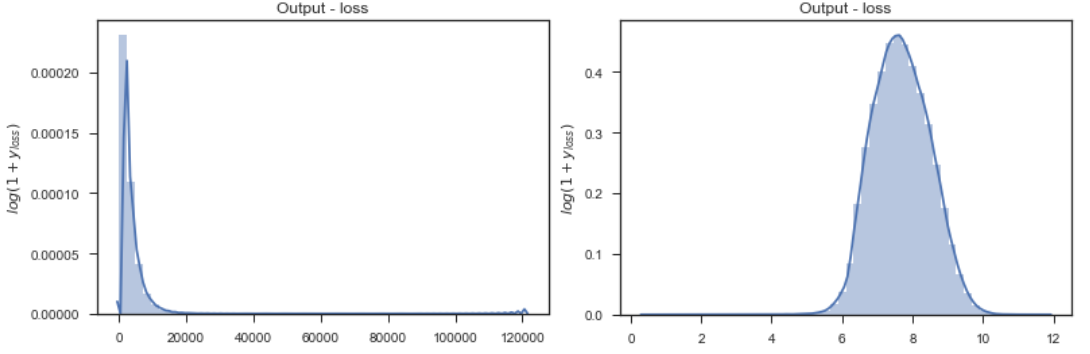
\includegraphics[width=.9\paperwidth]{Images/distribution-loss.png}}
\caption{Distribution plot of the output to the left and $log(1 + y_{loss})$ distribution to the right}
\label{fig:loss}
\end{figure}
\begin{figure}[H]
\centering
\makebox[\textwidth]{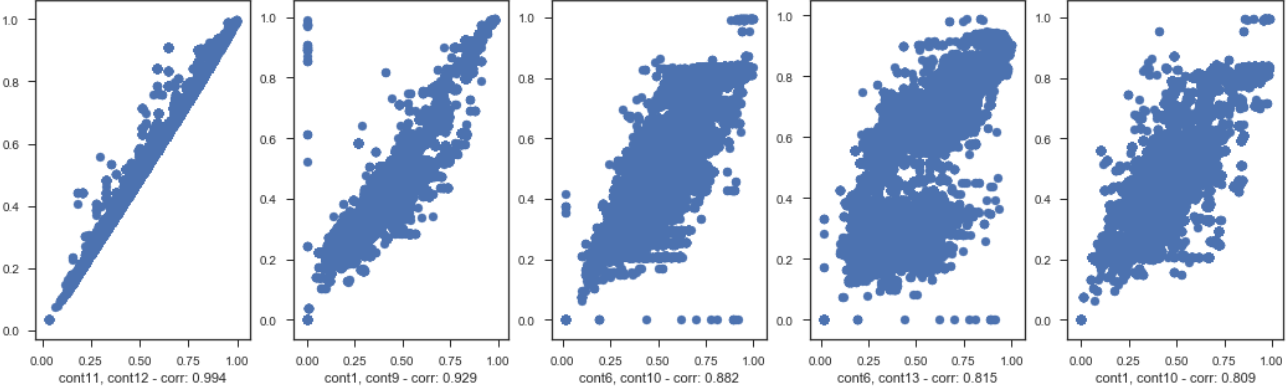
\includegraphics[width=.9\paperwidth]{Images/continuous-correlation.png}}
\caption{Five highest correlation pairs among continuous attributes}
\label{fig:con-corr}
\end{figure}
To start the modeling process a few test runs were executed with all of the models to get a feel of their respective potential. Since the output is highly skewed it was transformed with $y=log(1 + y)$ in order to correct for the skewness, assumed that the liner-models would then perform better. However the results obtained with log-transform were so far off that when executing the inverse with $x^y - 1$ resulted in overflow errors and thus making some of the experiments useless.  Some tests were performed using a TruncatedSVD instead of PCA (marked Test Error SVD), other tests were performed using reduced features, where the most relevant features were selected from a previously trained LassoLARSCV model.  The only cases where using this provided any improvement was when using Linear Regression, which was already known to be very sensitive to outliers.
The highly correlated pairs of attributes where tackled by removing one from each pair, thus removing ['cont9', 'cont12', 'cat2', 'cat3', 'cat4', 'cat5', 'cat6', 'cat7', 'cat8', 'cat86'].
\begin{table}[H]
\begin{tabular}{ |c|c|c|c|c|c|c| }
\hline
Model                     & Train Error & Test Error     &  PCA & NMF & SVD & RF \\
\hline
LinearRegression          & 1480        & 8.7e10 & 1336            & 1372 & 1242.29 & 1245.83 \\
Ridge                     & 1481        & 1477.830       & 1336            & 1367 & -       & -       \\
RidgeCV                   & 1242.29     & 1241.97        & -               & -    & 1245.68 & 1241.92 \\
Lasso                     & 1493        & 1481.435       & 1335            & 1380 &    -    &    -    \\
LassoCV                   & 1249        & 1245.15        & -               &  -   &    -    &    -    \\
LassoLARSCV               & 1245.98     & 1240.34        & -               & -    & 1244.54 &    -    \\
ElasticNet                & 1248.77     & 1244.99        & 1503            & 1969 & 1245.50 & 1246.94 \\
BaggingRegressor          & 605         & 1519.984       & 1385            & 1350 & -       &    -    \\
ETRegressor       & 0           & 1535.685       & 1379            & 1359 & -       &    -    \\
RFRegressor     & 602         & 1519.550       & 1390            & 1344 & -       &    -    \\
GBRegressor & 1453        & 1444.904       & 1317            & 1263 & -       &    -    \\
MLP                       & 1392        & 1410.916       & 1224            & 1363 & -       &    -    \\
KNRegressor       & 1364        & 1672.010       & -               & -    & -       &    -    \\
SVR                       & 1724        & 1755.613       & -               & -    & -       &    -    \\
\hline
\end{tabular}
\caption{\label{tab:start}The first tests, all models used the default Scikit-Learn parameters except GradientBoostingRegressor with loss='huber'}
\end{table}

The first test results are listed in table \ref{tab:start}. The MLP and the tree models give promising results, since they give the lowest test error even though they seem to have overfitted the training data. The training error for these models with PCA or NMF (with no column remove beforehand) applied to the data beforehand look promising as well for some of the models. The large deviation in improvement and in some cases even deterioration for the MNF transformation seems rather strange. \\\\
For the tree models a decision was made to study Gradient Boosting throughly since Scikit-Learn provides the Huber loss function \ref{eq:6} which is similar to MAE.
\begin{equation} \label{eq:6}
HuberLoss(y, \hat{y}) = \begin{cases} 
                  \frac{1}{2}(y - \hat{y})^2 & for\ |x|\leq \alpha \\
                  \alpha|y - \hat{y}|-\frac{1}{2}\alpha^2 & otherwise
               \end{cases}
\end{equation}
The Gradient Boosting has quite many parameters, in order to find the best combination of hyper-parameters a thorough grid scan was executed. The grid scan was executed for n\_estimators=[5, 50, 250, 500], alpha=[0.9, 0.5, 0.1], learning\_rate=[0.1, 0.0001], min\_samples\_leaf=[10, 20], min\_samples\_split=[10, 20] and max\_depth=[2, 3, 6]. The lowest mean absolute error of 1161 was obtained with (alpha=0.5, n\_estimators=250, max\_depth=6, learning\_rate=0.1, min\_samples\_leaf=20, min\_samples\_split=20), the results can be seen in figure~\ref{fig:gbr}. Extra parameter lop was executed for only the n\_estimators parameter, giving the most promising results with (alpha=0.5, n\_estimators=600, max\_depth=6, learning\_rate=0.1, min\_samples\_leaf=20, min\_samples\_split=20) with and MAE of 1142.

These set of parameters with the whole test dataset where used to predict the loss for the Kaggle submission. The results where rather disappointing with a MAE error of 1344. Attempt was made to improve this result by first applying NMF on the dataset and then using the Gradient Boosting model and as well with NMF on the dataset and $log(1 + y)$ on the output column. These attempts where speculated to improve the outcome based on the fact it improved in table \ref{tab:start} and the log transform was thought as to address the outliers better. However these attempts resulted in MAE of 1642 and 1625 respectively.  

Eventually, a GradientBoost regressor with  340 n\_estimators was trained using the training dataset using $loss=log(1 + y)$, and converting the predictions back using $loss_{pred} = e^{y_pred-1}$.  The resulting test set was submitted to kaggle and resulted in a mean absolute error of $1155.27344$.

\begin{figure}[H]
\centering
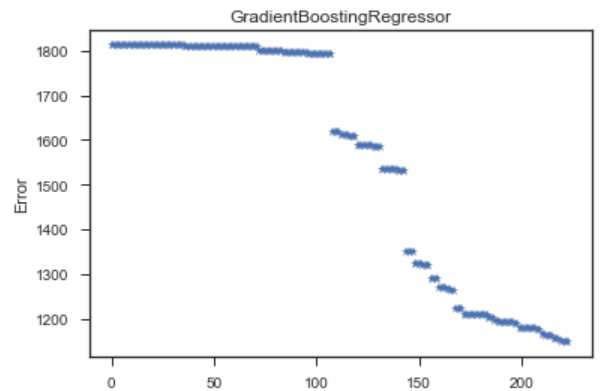
\includegraphics{Images/gbr.png}
\caption{Results for Gradient Boosting grid search}
\label{fig:gbr}
\end{figure}

A neural network was implemented using Keras/Tensorflow.  SKLearn's MLPRegressor was used at first, but Keras allows more fine-grained specification of various parameters of the problem, such as direct minimization of mean absolute error.  During training, a validation set is employed to measure improvement of training.  We opted to use rectified linear units (ReLU), as this appears to be the most favored method.  Various methods to determine the number of hidden layers and nodes were employed, but from early tests, it appeared that the first hidden layer should contain something between 400 and 600 nodes.  Using dropout apparently requires more than one hidden layer (although this is according to a google search), so the number of hidden layers was  set to 3, varying the size of the first hidden layer and the dropout percentage.  Setting the second and third layer to 50 and 10 appeared to give good results initially and was therefore chosen after some test runs with 1-3 hidden layers.

A big problem with the neural network proved to be overfitting, where the model gave a very low training error but the test error increased over time.  

To address this, two strategies were used, \textit{dropout}, and \textit{early stopping } combined with \textit{model checkpointing}. 

Dropout is a method in which  a neuron in a layer is blanked (\say{dropped out}) with a probability $p$ during each training stage.  This reduces the interdependency of neurons in that layer, and makes the whole network more robust towards overfitting.

Model checkpointing provides a method to save the state of the model every time an improvement of some metric is observed.  In our case, we were concerned with validation loss, i.e. the output of the loss function over the validation set, whenever an improvement is made, the whole model was saved to a file.  

Early stopping is a method to stop training of a neural network when a certain metric stops improving.  This was again used to halt training when validation loss no longer improved for $n_p$ epochs, where $n_p$ is a patience constant, set to 5 in our runs, i.e. when validation loss does not improve for 5 epochs, we halt.  

Using a combination of early stopping and model checkpointing allows us to use the model that performs best on the validation data set and throw away the results of overfitting.  Initial results with Keras were quite promising, so some time was spent to test various parameters.  Due to overfitting, one thing that was discovered was that increasing the number of epochs was not a very good way to increase improvement, but early stopping combined with checkpointing gave a lot better solution.  Training of 100 epochs or less was usually enough to trigger early stopping, i.e. the spot where validation loss started increasing while training loss still kept decreasing. See figure~\ref{fig:keras-overfitting}
\begin{figure}[H]
	\centering
	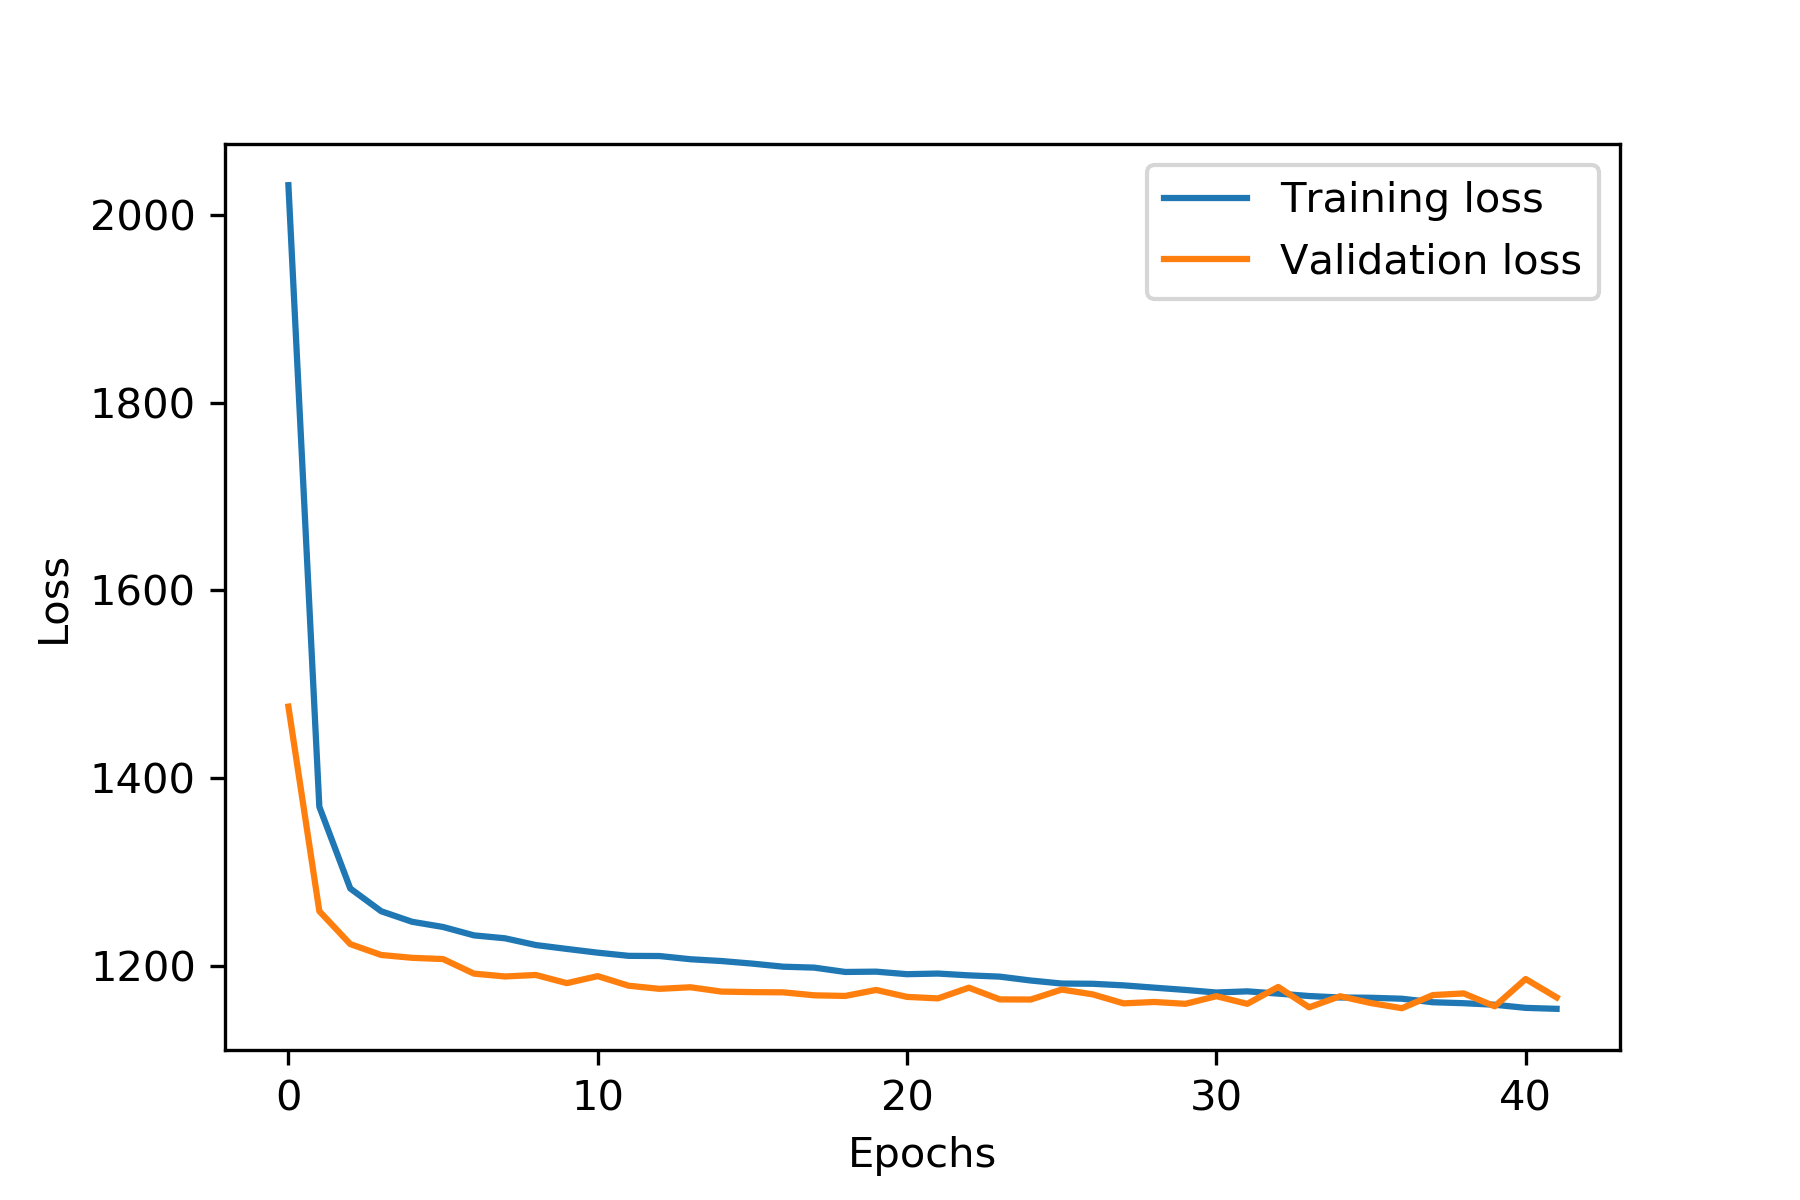
\includegraphics[width=15cm,height=8cm,keepaspectratio]{Images/keras-overfitting.png}
	\caption{Training loss and validation loss of a Keras/Tensorflow run, using early stopping.}
	\label{fig:keras-overfitting}
\end{figure}

Increasing dropout appears to make the loss curve sharper with changes in node count.  There appears to be a possible minimum between 400-450 nodes, and perhaps repeated iterations would help to find a better solution.  Figure~\ref{fig:keras-search} shows the best achieved test loss (on separate test set) for each combination.  There were multiple runs for each configuration, and the best result was always picked for the plot.

\begin{figure}[H]
	\centering
	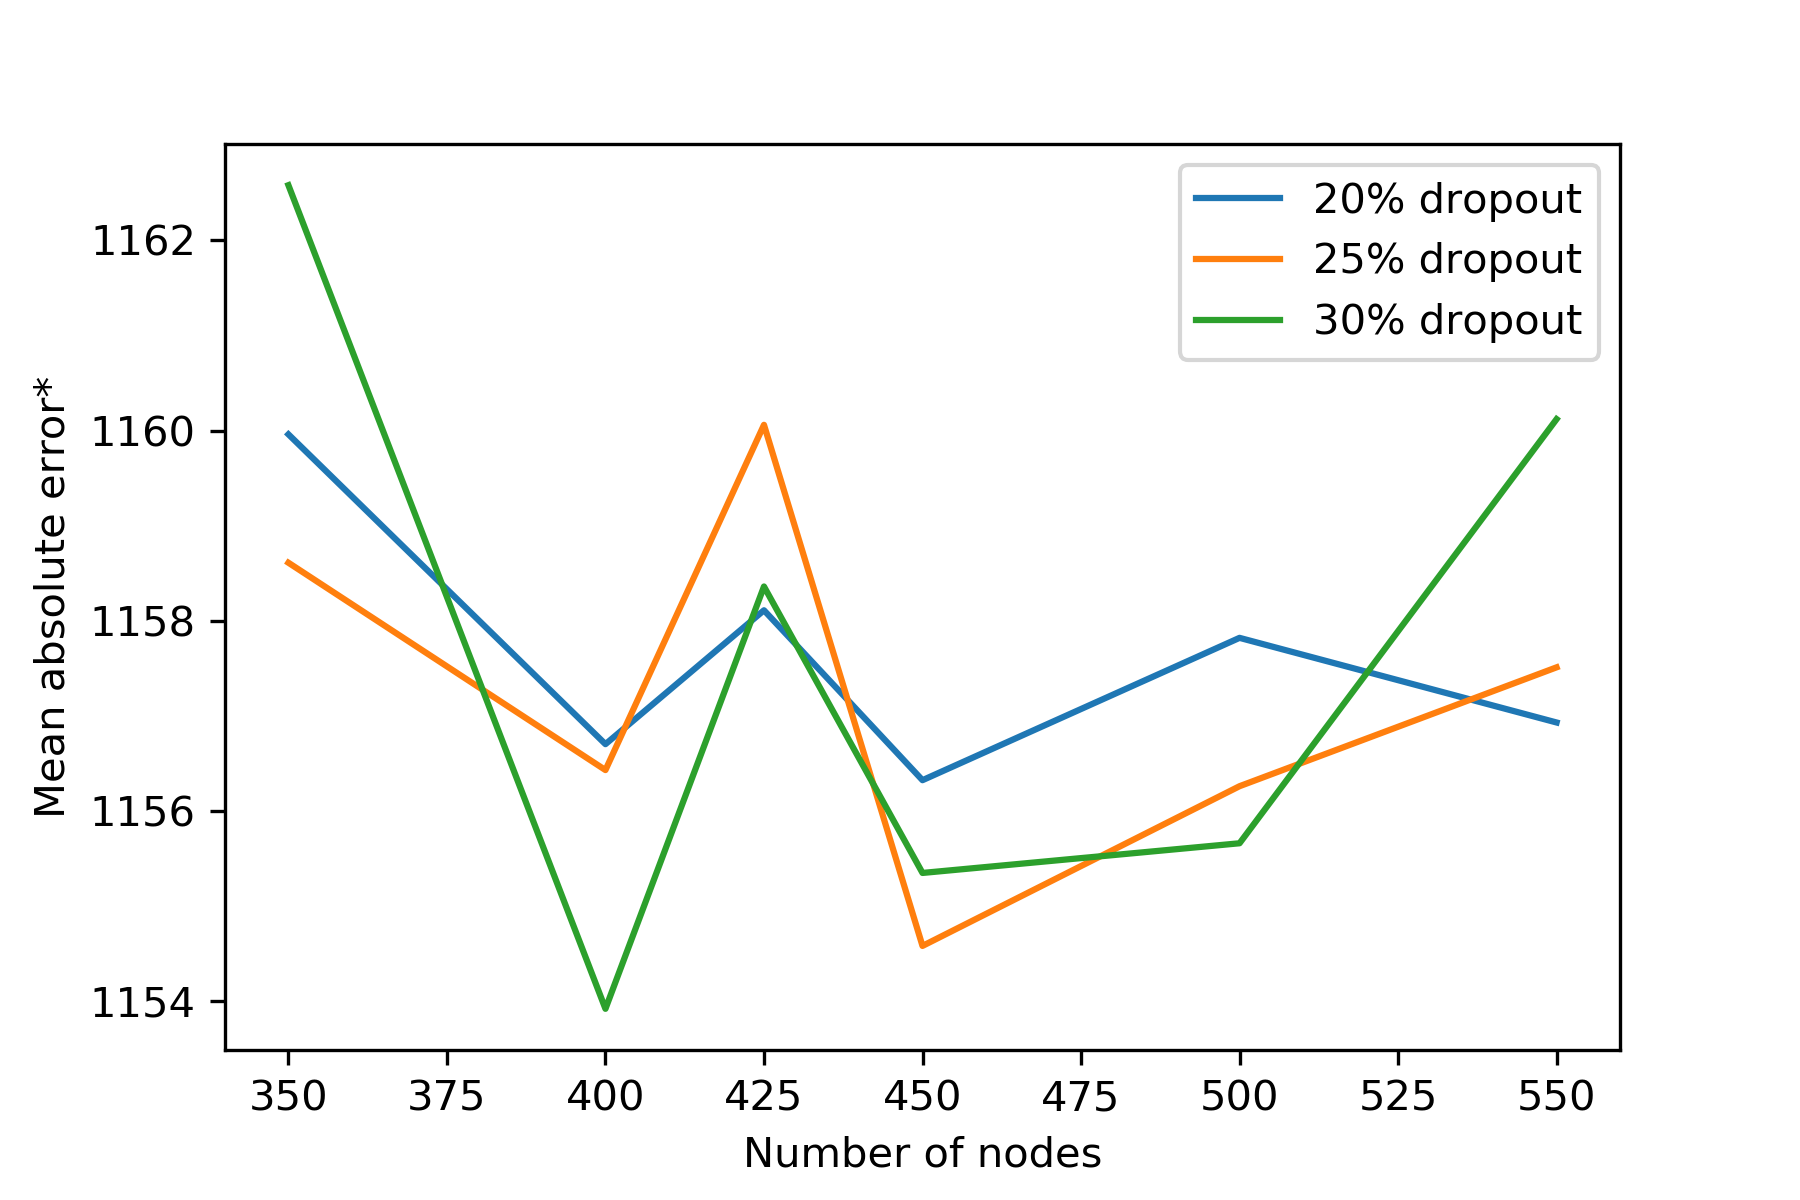
\includegraphics[width=15cm,height=8cm,keepaspectratio]{Images/keras-search.png}
	\caption{Results for Keras/TensorFlow grid search}
	\label{fig:keras-search}
\end{figure}

The best result was achieved via 400 nodes and a dropout percentage of 30\%, and gave 1139.33 as a score on Kaggle.


% * Fyrir verkefni #1 og #2: Töflur/myndir sem sýna t.d.
%   * Tíðnirit (e. histograms) fyrir stakar inntaksbreytur/úttaksbreytu, myndir sem sýna fylgni 2ja inntaksbreyta ofl.
%   * Nákvæmni einstakra líkana.
%   * Áhrif “hyperparametra” á gæði líkana.
%   * Yfirlit yfir inntaksbreytur sem mestu máli skipta.

% * Skrifið stutta lýsingu á því sem myndir og töflur sýna. Númerið allar myndir og töflur og notið númer þegar vísað er í úr texta (“Á mynd 2 má sjá …”) Gætið þess texti á myndum sé læsilegur (ekki of lítill).

% * Lýsið stuttlega tilraunum sem skiluðu litlu (“misheppnuðust”)

\section{Conclusion}

Our best results appear to have been reached using Keras/Tensorflow.  It appears that the input is somewhat codependent, and that the Neural Network, with dropout, is able to cope best out of the models investigated with that fact.  Feature reduction using various methods did not appear to improve the performance of other models, and neither did PCA.  

Future work would investigate better preprocessing, perhaps looking at feature construction methods.

The performance of Keras/TensorFlow neural networks warrants further investigation.  One thing that might be considered is to train such a neural network with the whole training set (rather than setting aside a test set), as the Keras neural network only utilizes a static validation set.  The downside to this would be that external validation would be subject to kaggle.com.

Gradient Boosting also performed well.  Perhaps this could be further investigated using XGBoost, which appears to be quite popular currently, especially for competitions.

Contributions were more or less equally divided.  Eggert worked primarily on Keras/Tensorflow and measuring some automated feature reduction methods.  Thor worked on Gradient Booster and analysis of feature contributions.
% * Helstu ályktanir.
% * Næstu skref. (Hvernig mynduð þið halda áfram með verkefnið?)

\appendix
\setlength{\voffset}{0cm}
\setlength{\hoffset}{0cm}

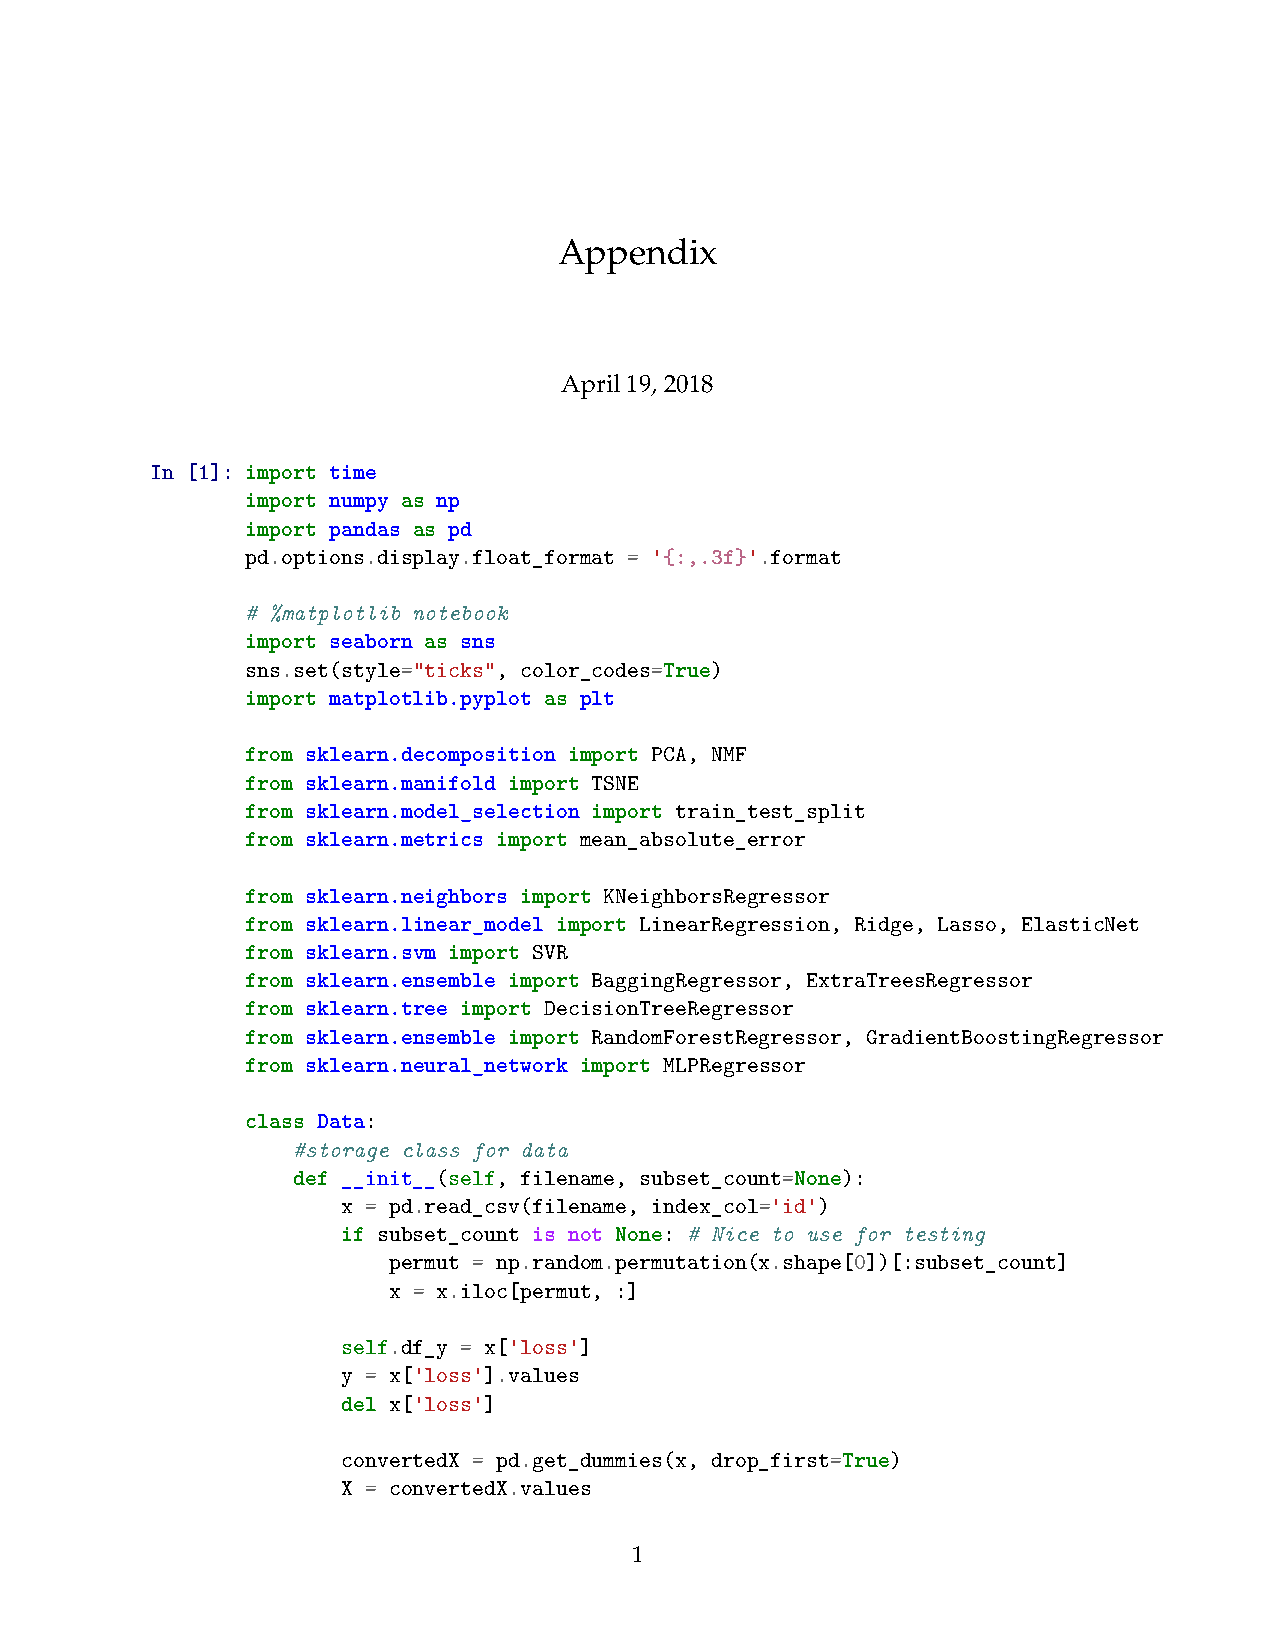
\includepdf[pages=-]{Images/Appendix.pdf}

\setlength{\voffset}{-2.54cm}
\setlength{\hoffset}{-2.54cm}

% For example, you can cite the Nano 3 Lecture notes \cite{nano3}.
% \newpage
% \begin{thebibliography}{9}
% \bibitem{nano3}
%   K. Grove-Rasmussen og Jesper Nygård,
%   \emph{Kvantefænomener i Nanosystemer}.
%   Niels Bohr Institute \& Nano-Science Center, Københavns Universitet
% \end{thebibliography}
\end{document}